\documentclass[11pt,a4paper]{article}
\usepackage{fontspec}
\usepackage{setspace}
\usepackage{amsmath,amsfonts,amssymb,amsthm}
\usepackage[margin=1.1in]{geometry}
\usepackage{graphicx}
\usepackage{subfigure}
\usepackage{listings}
\usepackage{booktabs,dcolumn}                     
\usepackage{fancyhdr}
\usepackage{bbm}
\usepackage{multirow}
\usepackage{booktabs}
\usepackage{harvard}
\usepackage{enumerate}
\newcommand{\ra}[1]{\renewcommand{\arraystretch}{#1}}
\DeclareMathOperator{\tr}{tr}
\DeclareMathOperator{\vect}{vec}
\makeatletter
\newcommand*{\rom}[1]{\expandafter\@slowromancap\romannumeral #1@}
\makeatletter

\setstretch{1.4}
\setlength{\headheight}{15pt} 
\graphicspath{{graphs/}}  

\newtheorem{sectheorem}{Example}

 
\begin{document}
\title{Applied Survival Analysis - January 2016\\Solutions to Lab 8: Parametric Survival Analysis}
\date{\vspace{-10ex}}
\author{\vspace{-10ex}}
\maketitle
We first import the data in \verb|R| and calculate the length of stay in years
\begin{spacing}{1.2}
\begin{footnotesize}
\begin{verbatim}
> ###########################################
> ### LAB 8: Parametric Survival Analysis ###
> ###########################################
> 
> # Import the data into R
> nurshome = read.csv("C:/Applied_Survival_Analysis_Jan2016/lab7/data/nurshome.csv")
> nurshome$losyr = nurshome$los/365
> head(nurshome)
  los age rx gender married health fail      losyr
1 665  83  1      0       0      4    1 1.82191781
2 697  80  0      0       0      3    0 1.90958904
3   7  92  1      0       0      4    1 0.01917808
4 217  69  0      0       0      3    1 0.59452055
5 153  74  1      1       0      3    1 0.41917808
6  54  85  0      0       0      4    1 0.14794521
\end{verbatim}
\end{footnotesize}
\end{spacing}
\begin{enumerate}[(i)]
\item We can use the function \verb|survreg| to fit parametric survival models. To fit an exponential model, we have to specify \verb|dist = "exp"|.
\begin{spacing}{1.2}
\begin{footnotesize}
\begin{verbatim}
> # (i): Fit an exponential model
> library(survival)
Loading required package: splines
> fitExp = survreg( Surv(losyr,fail) ~ gender,data = nurshome,dist = "exp")
> summary(fitExp)

Call:
survreg(formula = Surv(losyr, fail) ~ gender, data = nurshome, 
    dist = "exp")
              Value Std. Error     z        p
(Intercept) -0.0578     0.0333 -1.73 8.28e-02
gender      -0.5162     0.0619 -8.34 7.62e-17

Scale fixed at 1 

Exponential distribution
Loglik(model)= -1006.3   Loglik(intercept only)= -1038.4
	Chisq= 64.2 on 1 degrees of freedom, p= 1.1e-15 
Number of Newton-Raphson Iterations: 5 
n= 1591 

> 
> # corresponding cox model
> fitCox = coxph( Surv(losyr,fail) ~ gender,data = nurshome)
> summary(fitCox)
Call:
coxph(formula = Surv(losyr, fail) ~ gender, data = nurshome)

  n= 1591, number of events= 1269 

         coef exp(coef) se(coef)     z Pr(>|z|)    
gender 0.3958    1.4855   0.0621 6.373 1.85e-10 ***
---
Signif. codes:  0 ‘***’ 0.001 ‘**’ 0.01 ‘*’ 0.05 ‘.’ 0.1 ‘ ’ 1

       exp(coef) exp(-coef) lower .95 upper .95
gender     1.486     0.6732     1.315     1.678

Concordance= 0.541  (se = 0.006 )
Rsquare= 0.024   (max possible= 1 )
Likelihood ratio test= 38.29  on 1 df,   p=6.11e-10
Wald test            = 40.62  on 1 df,   p=1.852e-10
Score (logrank) test = 41.14  on 1 df,   p=1.415e-10
\end{verbatim}
\end{footnotesize}
\end{spacing}
We observe opposite signs between the results from the exponential model and the Cox model. This is expected since we see in the help file of \verb|survreg| that the survreg function uses an accelerated failure-time
parameterization. However, in today's notes we saw that the exponential and Weibull models have both PH and AFT parameterizations. For the exponential case, to transform the coefficients into a PH form, just type the following
\begin{spacing}{1.2}
\begin{footnotesize}
\begin{verbatim}
> # Tranform coefficients into a proportional hazards parameterization
> - coef(fitExp)
(Intercept)      gender 
 0.05775499  0.51618597 
\end{verbatim}
\end{footnotesize}
\end{spacing}
\item Now we'd like to plot the survival curves predicted by the exponential model, along with the raw KM estimates.
\begin{spacing}{1.2}
\begin{footnotesize}
\begin{verbatim}
# Get the KM estimates
fitKM = survfit( Surv(losyr,fail) ~ gender,data = nurshome)

# (ii): Comparing exponential model with KM
setwd("C:/Applied_Survival_Analysis_Jan2016/lab8/graphs")

pdf("ExpKM.pdf",height = 5.5, width = 5.5)
plot(fitKM,mark.time = F,main = "Predicted survival for Exponential model VS KM",
     xlab = "Length of Stay (years)",ylab = "Survival probability",lty = 1:2,
     col = c("blue","red"))
# Add the curves fitted by the exponential model
pct = seq(0,1,by = 0.001)
lines(predict(fitExp,newdata = data.frame(gender = 0),type = "quantile",
              p = pct),1-pct,lty = 3,col = "green")
lines(predict(fitExp,newdata = data.frame(gender = 1),type = "quantile",
              p = pct),1-pct,lty = 4,col = "orange")
legend("topright",bty = "n",lty = 1:4,col = c("blue","red","green","orange"),
       legend = c("KM: Females","KM: Males","EXP: Females","EXP: Males"),ncol = 2)
dev.off()
\end{verbatim}
\end{footnotesize}
\end{spacing}
\begin{figure}[htbp]
	\centering
		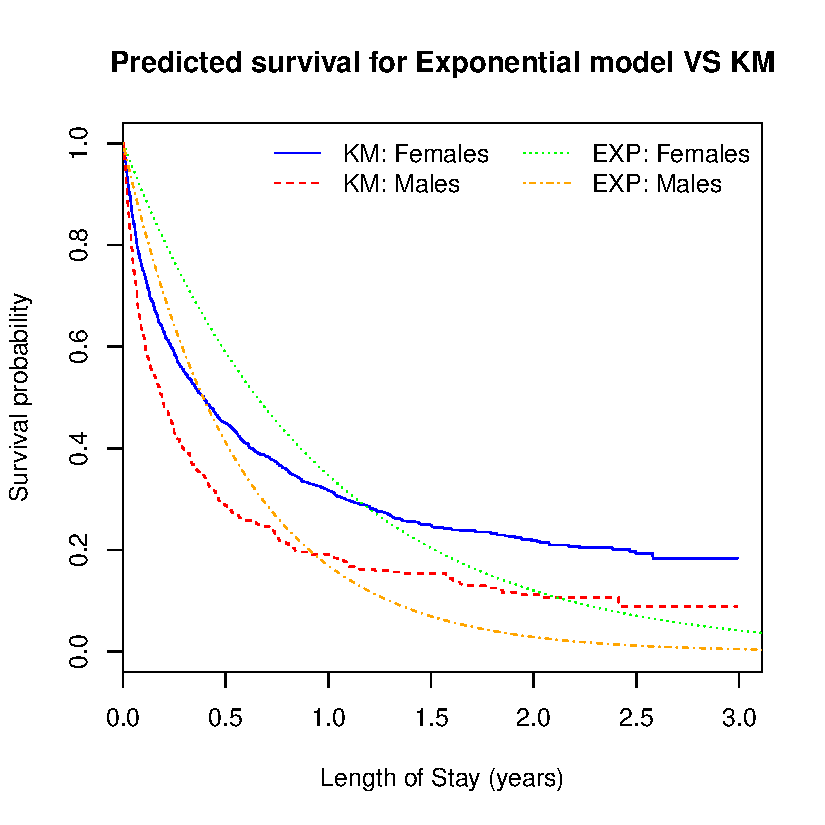
\includegraphics[scale=0.9]{ExpKM.pdf}
		%\rule{35em}{0.5pt}
	\caption{Exponential Model by Gender.}
	\label{figure1}
\end{figure}
It seems that there is a discrepancy between the exponential model and the KM estimates. Thus, we feel that the exponential model is unlikely to fit the data well. 

Now, let's examine the previous code in more detail. First, we save the KM estimates by gender in the object \verb|fitKM|. Then we use the \verb|plot| function to plot the KM estimates for males and females. However, we would also like to add the curves predicted by the exponential model on the graph. To do so, we use the function \verb|lines| (see \verb|?lines|). On the y-axis we have the survival probabilities from 1 to 0 with the increment of the sequence being 0.001 (please, see \verb|?seq|)
\begin{spacing}{1.2}
\begin{footnotesize}
\begin{verbatim}
> pct = seq(0,1,by = 0.001)
> 1-pct[c(1:5,998:1001)]
[1] 1.000 0.999 0.998 0.997 0.996 0.003 0.002 0.001 0.000
\end{verbatim}
\end{footnotesize}
\end{spacing}
and using the \verb|predict| function (please, see \verb|?predict.survreg|)
\begin{spacing}{1.2}
\begin{footnotesize}
\begin{verbatim}
predict(fitExp,newdata = data.frame(gender = 0),type = "quantile",
        p = pct)
\end{verbatim}
\end{footnotesize}
\end{spacing}  
we get the survival times at which the survival probabilities \verb|1-pct| (i.e., $1, 0.999, \ldots,0$) correspond. The reason for this odd syntax is that the \verb|predict| function returns the vector of quantiles of the distribution function $F(t) = 1 - S(t)$ (more in class if needed). 
\item We now fit a corresponding Weibull model using the \verb|survreg| function with the option \verb|dist = "weibull"|
\begin{spacing}{1.2}
\begin{footnotesize}
\begin{verbatim}
> # (iii): Fit a Weibull model
> fitWei = survreg( Surv(losyr,fail) ~ gender,data = nurshome,dist = "weibull")
> summary(fitWei)

Call:
survreg(formula = Surv(losyr, fail) ~ gender, data = nurshome, 
    dist = "weibull")
             Value Std. Error     z        p
(Intercept) -0.143     0.0542 -2.65 8.13e-03
gender      -0.673     0.1011 -6.66 2.67e-11
Log(scale)   0.487     0.0232 20.99 8.94e-98

Scale= 1.63 

Weibull distribution
Loglik(model)= -731.1   Loglik(intercept only)= -751.9
	Chisq= 41.73 on 1 degrees of freedom, p= 1e-10 
Number of Newton-Raphson Iterations: 5 
\end{verbatim}
\end{footnotesize}
\end{spacing}
The model is fitted in the accelerated failure-time metric, and thus, to get the estimates in the log relative-hazard metric use the following code
\begin{spacing}{1.2}
\begin{footnotesize}
\begin{verbatim}
> # Tranform coefficients into a proportional hazards parameterization
> - coef(fitWei)/fitWei$scale
(Intercept)      gender 
 0.08814507  0.41380822
\end{verbatim}
\end{footnotesize}
\end{spacing}
Now we'd like to produce a graph that compares the survival curves predicted by the Weibull model with the raw KM survival estimates
\begin{spacing}{1.2}
\begin{footnotesize}
\begin{verbatim}
> # Comparing Weibull model with KM
> pdf("WeiKM.pdf",height = 5.5, width = 5.5)
> plot(fitKM,mark.time = F,main = "Predicted survival for Weibull model VS KM",
+      xlab = "Length of Stay (years)",ylab = "Survival probability",lty = 1:2,
+      col = c("blue","red"))
> # Add curves fitted by the Weibull model
> pct = seq(0,1,by = 0.001)
> lines(predict(fitWei,newdata = data.frame(gender = 0),type = "quantile",
+               p = pct),1-pct,lty = 3,col = "green")
> lines(predict(fitWei,newdata = data.frame(gender = 1),type = "quantile",
+               p = pct),1-pct,lty = 4,col = "orange")
> legend("topright",bty = "n",lty = 1:4,col = c("blue","red","green","orange"),
+        legend = c("KM: Females","KM: Males","WEI: Females","WEI: Males"),ncol = 2)
> dev.off()
RStudioGD 
        2 
\end{verbatim}
\end{footnotesize}
\end{spacing}

\begin{figure}[htbp]
	\centering
		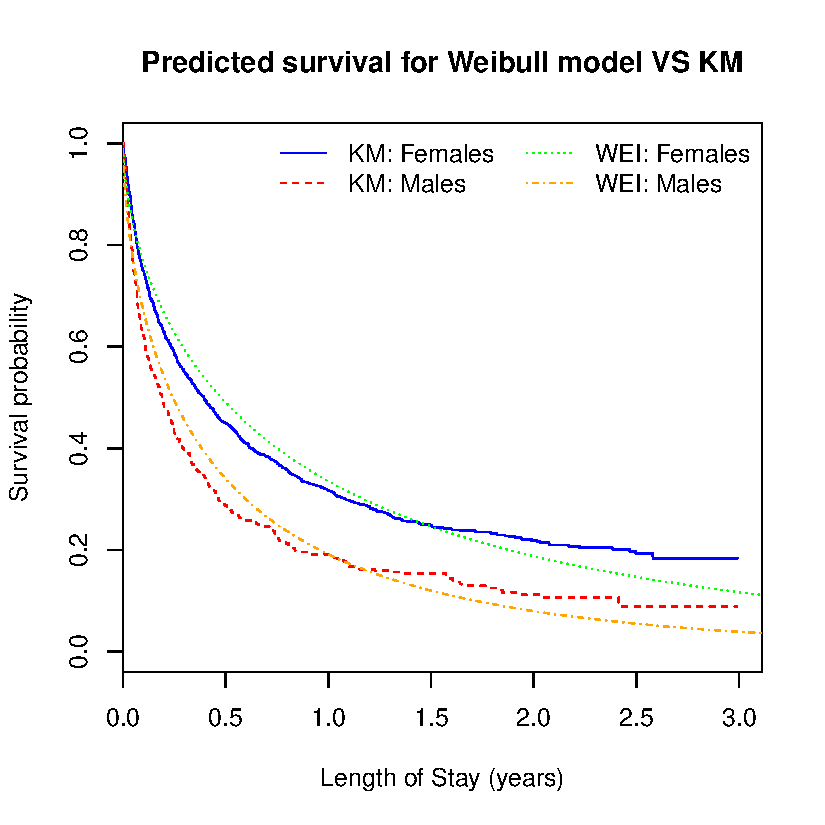
\includegraphics[scale=0.9]{WeiKM.pdf}
		%\rule{35em}{0.5pt}
	\caption{Weibull Model by Gender.}
	\label{figure2}
\end{figure}
It seems that the Weibull model fits the data much better than the exponential model, but we are still not happy with the model fit.
\item Recall that the survival function of a Weibull distribution is
$S(t) = \exp\{-\lambda t^{\kappa}\}$, thus
\begin{align}
\Lambda(t) &= - \log S(t) = \lambda t^{\kappa} \Rightarrow \nonumber \\
\log(\Lambda(t)) &= \log(\lambda) + \kappa\log(t) \nonumber
\end{align}
So, we can plot $\log\Lambda(t)$ versus $\log(t)$ for each subgroup, and if it seems to form a straight line in $\log(t)$ (for each subgroup), then the Weibull distribution will be probably appropriate
for our dataset. 
Thus, we can focus on two different aspects of a log-cumulative hazard plot
\begin{itemize}
\item If the curves seem to be parallel, the PH assumption should be probably correct.
\item If the curves not only seem to be parallel but also seem to form a straight line, then the Weibull distribution along with the PH assumption will be appropriate.
\end{itemize}
\begin{figure}[htbp]
	\centering
		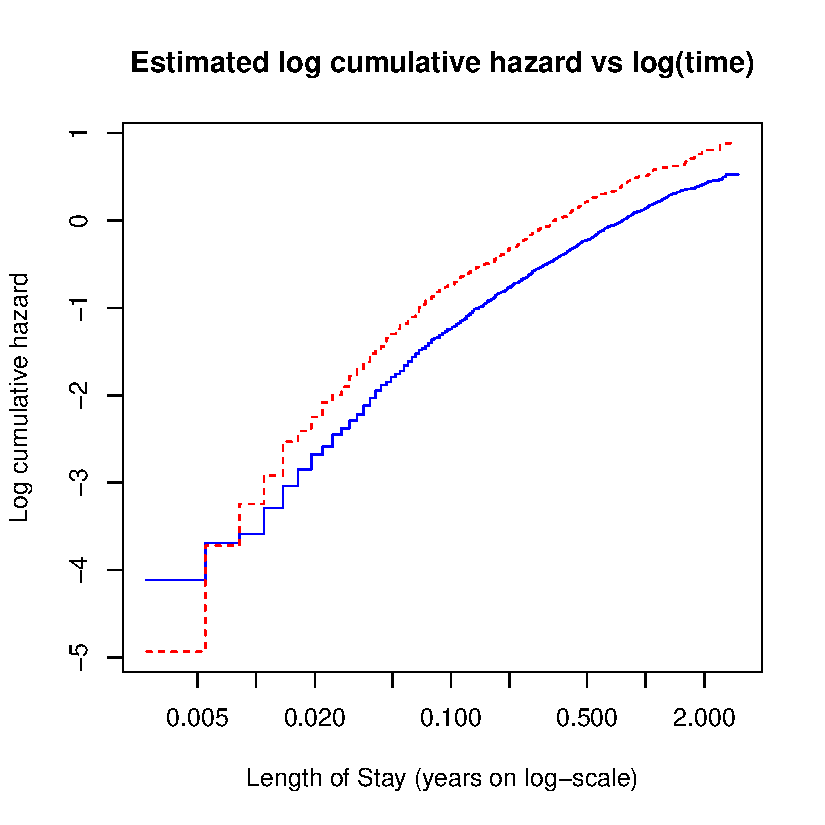
\includegraphics[scale=0.9]{logChaz.pdf}
		%\rule{35em}{0.5pt}
	\caption{Log cumulative hazard plot by Gender.}
	\label{figure3}
\end{figure}

If the Weibull assumption were appropriate, we would expect two straight lines on the graph above. However, since we can see that there is some curvature in the curves above, the Weibull distribution is unlikely to be appropriate for our dataset.   
\item We want to predict the mean and median length of stay for each gender according to the 
exponential and Weibull model. We know that for the exponential model the mean and the median are the following:
\begin{align}
\text{Mean} = 1/\lambda, \quad \text{Median} = -\dfrac{\log(0.5)}{\lambda},
\nonumber
\end{align} 
and for the Weibull model are the following:
\begin{align}
\text{Mean} = \lambda^{-1/\kappa}\Gamma[1/\kappa+1], \quad \text{Median} = \left[-\dfrac{\log(0.5)}{\lambda}\right]^{1/\kappa}.
\nonumber
\end{align} 
Thus, using \verb|R| code we get that
\begin{spacing}{1.2}
\begin{footnotesize}
\begin{verbatim}
> # (v): Mean and median times
> ExpModel = data.frame(Mean = rep(NA,2),Median = rep(NA,2)) 
> rownames(ExpModel) = c("Females","Males")
> 
> # Coefficients in PH form
> beta = - coef(fitExp)
> 
> ExpModel[,1] = 1/exp(cumsum(beta))
> ExpModel[,2] = - log(0.5)/exp(cumsum(beta))
> ExpModel
             Mean    Median
Females 0.9438812 0.6542486
Males   0.5633011 0.3904506
> 
> # Weibull model
> WeiModel = data.frame(Mean = rep(NA,2),Median = rep(NA,2)) 
> rownames(WeiModel) = c("Females","Males")
> 
> # Coefficients in PH form
> beta = - coef(fitWei)/fitWei$scale
> kappa = 1/fitWei$scale
> 
> WeiModel[,1] = gamma(1/kappa + 1)*exp(cumsum(beta))^(-1/kappa)
> WeiModel[,2] = (- log(0.5)/exp(cumsum(beta)) )^(1/kappa)
> WeiModel
             Mean    Median
Females 1.2646385 0.4771348
Males   0.6448826 0.2433074
\end{verbatim}
\end{footnotesize}
\end{spacing}
\newpage
\item \textbf{Optional:} First we construct the \verb|R| function to be used to compute the loglikelihood of the Weibull model
\begin{spacing}{1.2}
\begin{footnotesize}
\begin{verbatim}
> # (vi): Computing the loglikelihood for the Weibull model
> f = function(param)
+ {
+   # x: design matrix including the intercept
+   p = ncol(x)
+   
+   # Param: The parameter vector
+   beta = param[1:p]
+   kappa = param[p+1]
+   
+   lambda = exp(x%*%beta)
+   
+   logl = sum(delta*(log(kappa) + log(lambda) + (kappa-1)*log(time)) - lambda*time^kappa)
+   
+   return(-logl)
+ }
> 
> # Fit the weibull model
> fitWei = survreg( Surv(losyr,fail) ~ gender,data = nurshome,dist = "weibull")
> 
> # Tranform coefficients into a proportional hazards parameterization
> beta = - coef(fitWei)/fitWei$scale
> kappa = 1/fitWei$scale
> x = cbind(1,nurshome$gender)
> time = nurshome$losyr
> delta = nurshome$fail
> 
> # Compare
> f(c(beta,kappa))
[1] 731.0688
> fitWei$loglik[2]
[1] -731.0688
> 
> f(c(beta,kappa)) + fitWei$loglik[2]
[1] -3.183231e-12
\end{verbatim}
\end{footnotesize}
\end{spacing}
The results from the two likelihoods are essentially the same. Note that our function returns $-\log(L)$.

The \verb|nlm| is very useful for obtaining maximum likelihood estimates of a model. All we need to do is to pass our function in \verb|nlm|. Note that \verb|nlm| carries out a minimization of our function (therefore maximization of the likelihood) using a Newton-type algorithm. The derivatives required for the implementation of the algorithm are calculated numerically (see \verb|?nlm| for more details). The procedure requires some arbitrary starting values for the parameters. Let's start with $\boldsymbol{\beta} = (0,0)^{T}$ and $\kappa = 1$ (exponential model).
\begin{spacing}{1.2}
\begin{footnotesize}
\begin{verbatim}
> # Use the nlm function to maximize the loglikelihood
> # Starting values
> starting = c(rep(0,2),1)
> 
> nlm(f,starting,gradtol = 1e-10)
$minimum
[1] 731.0688

$estimate
[1] 0.08814452 0.41380802 0.61443847

$gradient
[1] -1.932676e-06 -5.115908e-06  9.890755e-06

$code
[1] 2

$iterations
[1] 14

Warning messages:
1: In log(kappa) : NaNs produced
2: In nlm(f, starting, gradtol = 1e-10) :
  NA/Inf replaced by maximum positive value
3: In log(kappa) : NaNs produced
4: In nlm(f, starting, gradtol = 1e-10) :
  NA/Inf replaced by maximum positive value
5: In log(kappa) : NaNs produced
6: In nlm(f, starting, gradtol = 1e-10) :
  NA/Inf replaced by maximum positive value
> beta;kappa
(Intercept)      gender 
 0.08814507  0.41380822 
[1] 0.614439
\end{verbatim}
\end{footnotesize}
\end{spacing}   
The results were almost the same, which means that we got the correct answer from \verb|nlm|. However, see the warning messages above. A better approach would be to maximize the likelihood with respect to $\log(\kappa)$, which is defined on the whole real line. As an example, you can see if this transformation speeds up the convergence of the algorithm, modifying the function \verb|f| accordingly.  


\end{enumerate}

 
\end{document}